\documentclass[conference]{IEEEtran}
% \IEEEoverridecommandlockouts
% The preceding line is only needed to identify funding in the first footnote. If that is unneeded, please comment it out.
\usepackage{cite}
\usepackage{amsmath,amssymb,amsfonts}
\usepackage{algorithmic}
\usepackage{graphicx}
\usepackage{float}
\usepackage{textcomp}
\usepackage{xcolor}
\usepackage{hyperref}
\def\BibTeX{{\rm B\kern-.05em{\sc i\kern-.025em b}\kern-.08em
    T\kern-.1667em\lower.7ex\hbox{E}\kern-.125emX}}

% GitHub link
\newcommand{\githublink}{\url{https://github.com/himangg/Cuisine-Recommendation-System}}

\begin{document}

\title{Cuisine Recommendation System}

\author{\IEEEauthorblockN{1\textsuperscript{st} Himang Chandra Garg}
\IEEEauthorblockA{\textit{Computer Science and Engineering} \\
\textit{Indraprastha Institute of Information Technology}\\
Roll no.- 2022214 \\
himang22214@iiitd.ac.in}
\and
\IEEEauthorblockN{2\textsuperscript{nd} Nishil Agarwal}
\IEEEauthorblockA{\textit{Computer Science and Artificial Intelligence} \\
\textit{Indraprastha Institute of Information Technology}\\
Roll no.- 2022334 \\
nishil22334@iiitd.ac.in}
}

\maketitle

\begin{abstract}
 In this report, we present the design and implementation of a cuisine recommendation system aimed at assisting users in discovering recipes that align with their tastes and dietary requirements. Leveraging machine learning techniques such as content-based and collaborative filtering, our system analyzes user preferences, ingredient profiles, and historical interactions to generate personalized recipe suggestions.
\end{abstract}

% GitHub link
\section{GitHub Repository}
The source code for our project can be found at: \githublink

\section{Problem being addressed}
The problem being addressed in this project is the need for a robust cuisine recommendation system that can assist users in discovering recipes aligned with their tastes, preferences, and dietary requirements. With the vast amount of recipe data available online, users often struggle to find recipes that suit their specific needs and interests. Additionally, users may also desire personalized recommendations based on their past interactions and feedback.


\section{Relevant Literature}

Existing research in cuisine recommendation systems has focused on collaborative filtering, content-based filtering, and hybrid approaches. However, these methods face challenges such as sparsity of user-item interaction data, limited diversity in recommendations, and scalability issues. The cold-start problem remains a key challenge, especially for new users or items with sparse data. Future research should aim to address these limitations by developing more effective recommendation techniques, enhancing diversity in recommendations, and improving scalability and efficiency. Also, there is no significant way to evaluate the accuracy of the recommendations. We have tried to do so by using a cosine similarity heatmap and precision at k. Additionally, advancements in deep learning, natural language processing, and user modeling can offer new opportunities for enhancing the accuracy, diversity, and personalization of recipe recommendations.

\section{Dataset}
% Details about the dataset used
For our project, we utilize a comprehensive dataset from Kaggle, comprising a diverse collection of Food recipes showcasing various regional cuisines and culinary traditions. The dataset includes essential information such as recipe names, ingredients, preparation time, nutritional content, and user ratings. In the earlier deadline we stated that we will be using.
https://www.kaggle.com/datasets/kritirathi/indian-food-dataset-with/data
but due to less rows we have changed our dataset to https://www.kaggle.com/datasets/irkaal/foodcom-recipes-and-reviews.

\section{Data Preprocessing}

In this section, we detail the preprocessing steps applied to the recipe dataset to prepare it for further analysis and modeling.

\subsection{Reading and Filtering Dataset}

The recipe dataset is initially read using the Pandas library, loading it into a DataFrame named \texttt{data}. Subsequently, irrelevant columns are filtered out to focus on essential attributes relevant to the recommendation system to reduce noise prevent unnecessary complexity.

\subsection{Removing Unnecessary Rows and Columns}

To enhance data consistency, we removed entries with missing ratings, incorrect/erroneous data etc. using the \texttt{drop} function.

\subsection{Selecting Diverse Rating Dishes}

Further, we stratified the dataset based on aggregated ratings, selecting a balanced mix of highly rated and lower-rated recipes for model training.

\subsection{Modifying Column Formats, Handling Missing and Erroneous Data}

 Additionally, we brought the entries of date\_of\_publication, cooking\_time, ingredients  columns into the required format for efficient handling of data. We also handled missing values in various columns, ensuring consistency and completeness.

\subsection{Removing Duplicate Entries}

Duplicate recipe names are removed from the dataset, ensuring uniqueness and avoiding redundancy in recommendations.

\subsection{Merging Datasets}

The preprocessed recipe dataset is merged with the reviews dataset based on \texttt{RecipeId}, facilitating the integration of user ratings into the recommendation system.

\subsection{Filtering Reviews}

Reviews from reviewers with less than five reviews are removed from the dataset, ensuring that only substantial reviews are considered in the analysis.

\subsection{Saving Processed Data}

The final preprocessed dataset is saved to a new file for further analysis and modeling.

\section{Data Visualization}

In this section, we present visualizations of various aspects of the processed dataset to gain insights into recipe categories, rating distribution, publication trends, calorie distribution, and top recipes and authors based on review count.

\subsection{Distribution of Recipe Categories}

The distribution of recipe categories is visualized using a pie chart. Rare categories, representing less than 1 percent of the dataset, are grouped under 'Others' to simplify the visualization.

\begin{figure}[H]
\centering
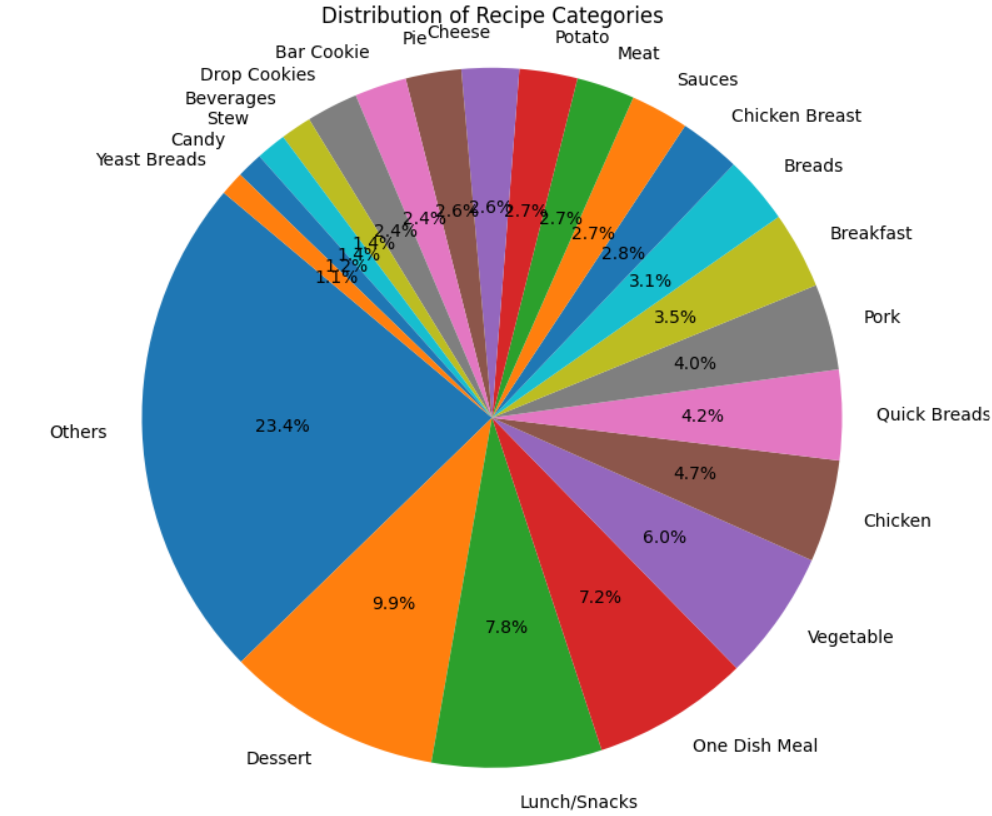
\includegraphics[width=0.4\textwidth]{1.png}
\caption{Distribution of Recipe Categories}
\label{fig:distribution_categories}
\end{figure}

\subsection{Distribution of All Ratings}

A count plot is used to visualize the distribution of all ratings. This plot provides an overview of the distribution of ratings assigned to recipes in the dataset.

\begin{figure}[H]
\centering
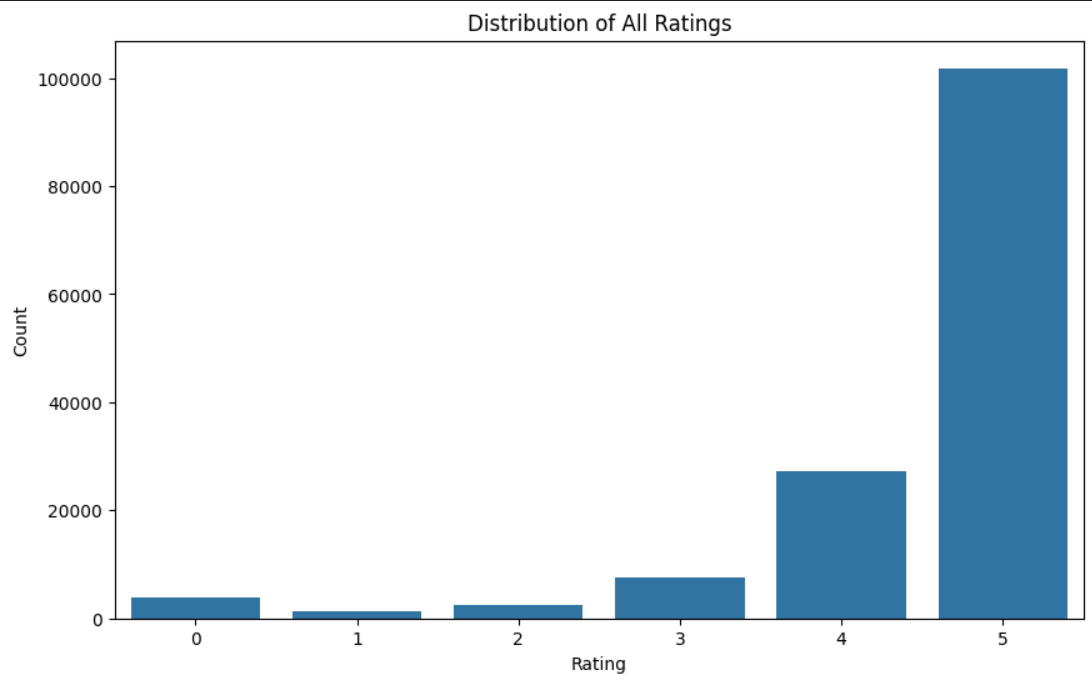
\includegraphics[width=0.4\textwidth]{2.png}
\caption{Distribution of All Ratings}
\label{fig:distribution_ratings}
\end{figure}


\subsection{Monthly Recipe Publication}

A line plot is utilized to illustrate the monthly publication of recipes over time. This visualization helps identify trends and patterns in recipe publication frequency.

\begin{figure}[H]
\centering
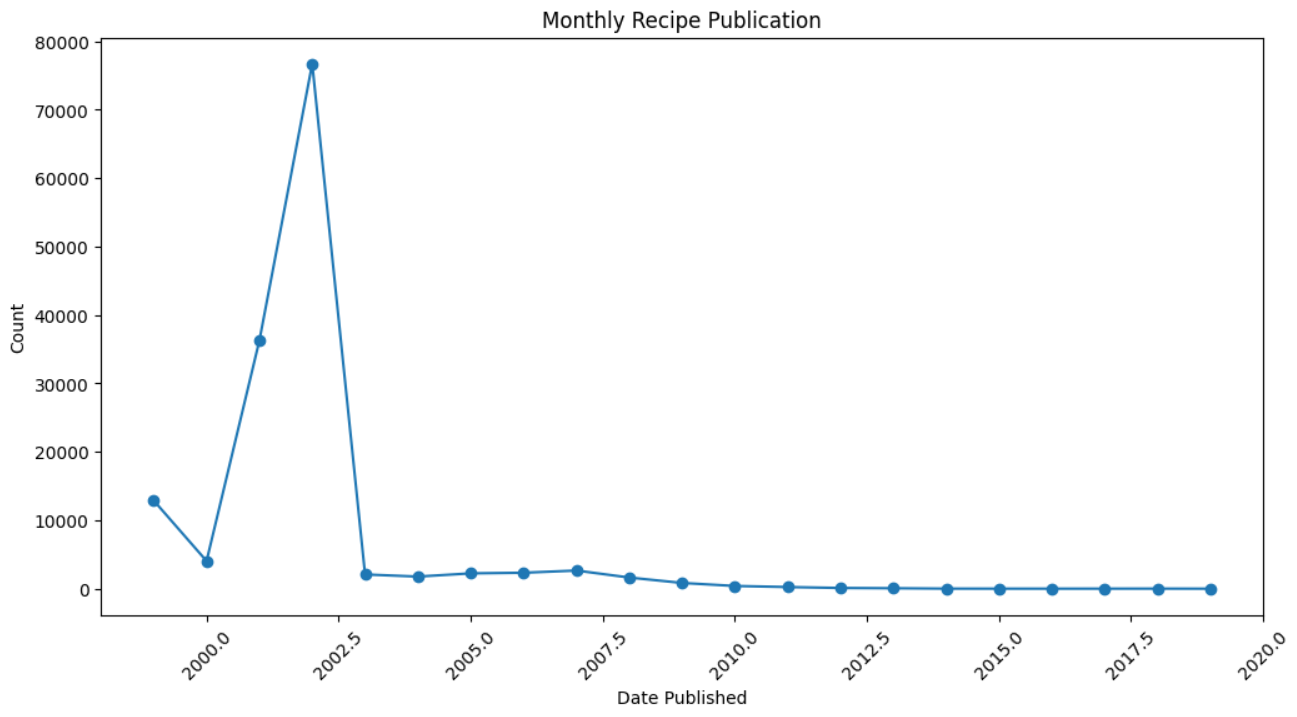
\includegraphics[width=0.4\textwidth]{3.png}
\caption{Monthly Recipe Publication}
\label{fig:monthly_publication}
\end{figure}

\subsection{Distribution of Calories}

The distribution of calories in recipes is displayed using a pie chart, categorizing calorie ranges into bins. This visualization offers insights into the distribution of calorie content across recipes.

\begin{figure}[H]
\centering
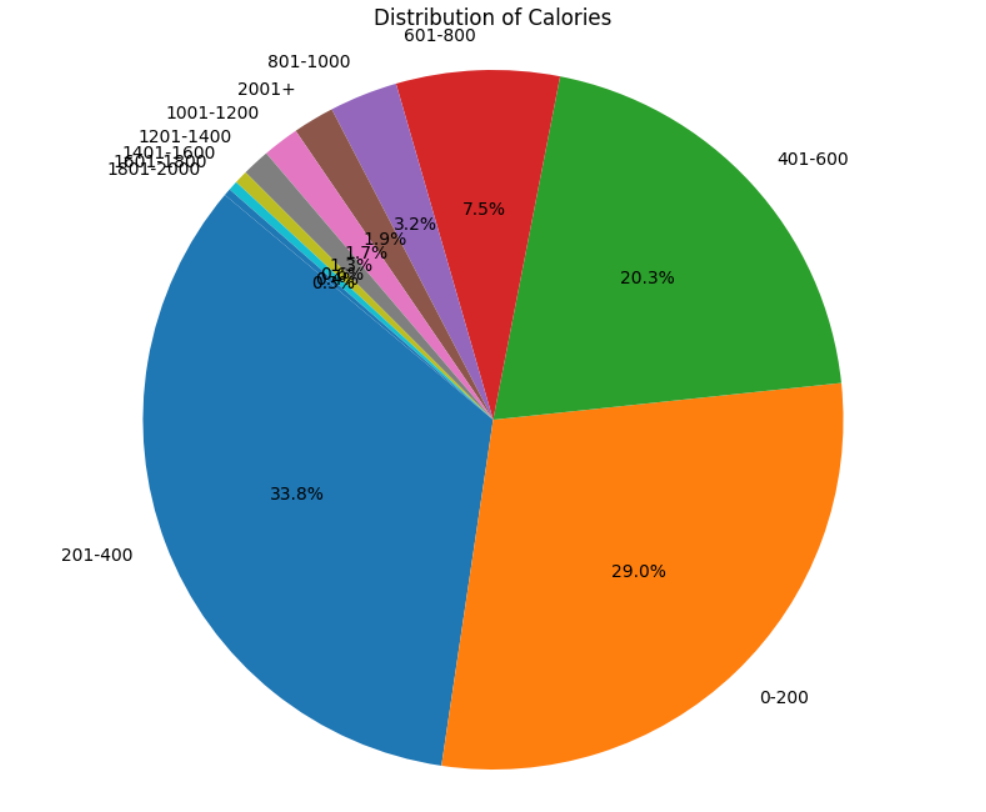
\includegraphics[width=0.4\textwidth]{4.png}
\caption{Distribution of Calories}
\label{fig:distribution_calories}
\end{figure}

\subsection{Top 10 Recipes by Review Count}

A bar plot is employed to showcase the top 10 recipes based on review count. This visualization highlights recipes that have received the highest number of reviews from users.

\begin{figure}[H]
\centering
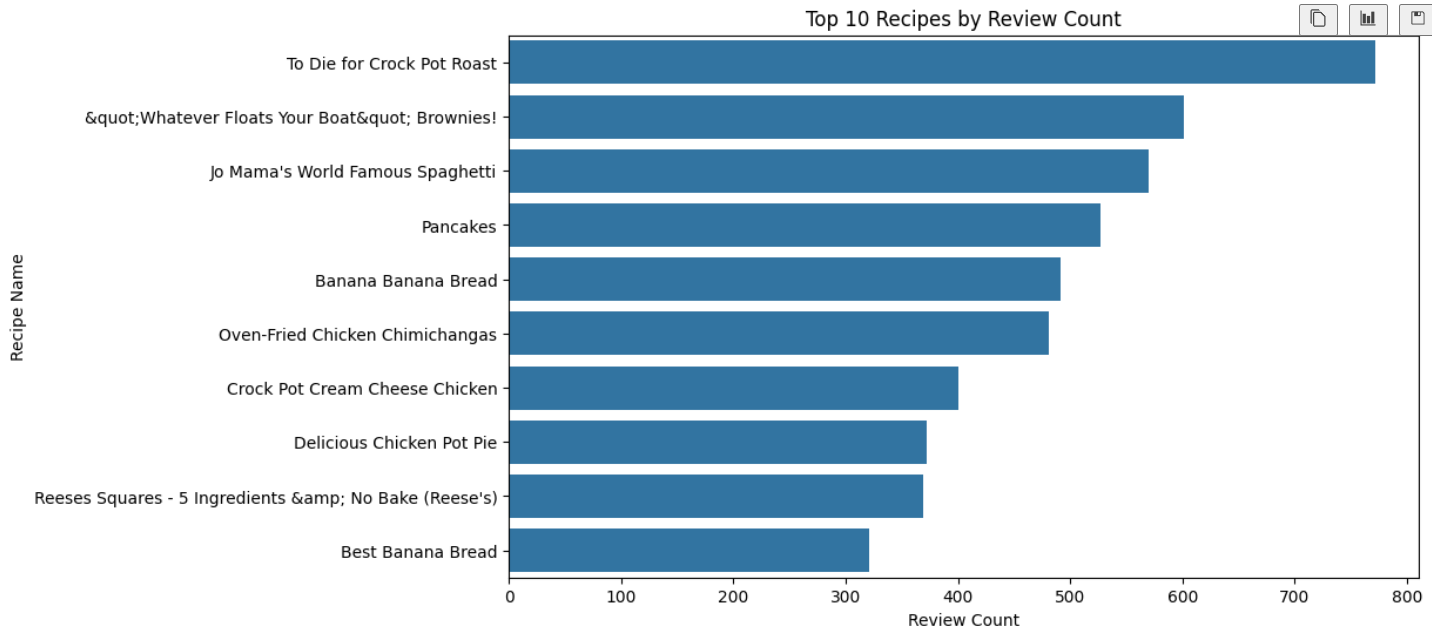
\includegraphics[width=0.4\textwidth]{5.png}
\caption{Top 10 Recipes by Review Count}
\label{fig:top10_recipes}
\end{figure}

\subsection{Top 10 Authors by Review Count}

Similarly, a bar plot is utilized to present the top 10 authors based on review count. This visualization identifies authors who have contributed the most reviewed recipes in the dataset.

\begin{figure}[H]
\centering
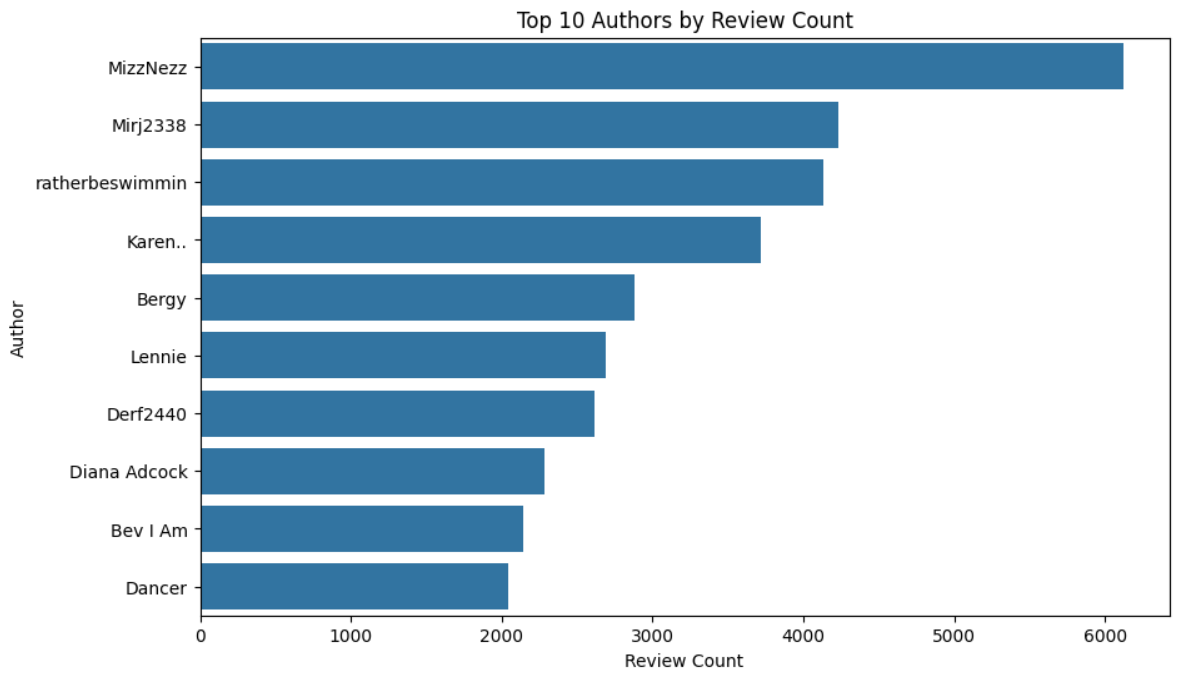
\includegraphics[width=0.4\textwidth]{6.png}
\caption{Top 10 Authors by Review Count}
\label{fig:top10_authors}
\end{figure}

Each visualization offers valuable insights into different aspects of the recipe dataset, aiding in understanding user preferences, recipe popularity, and publication trends.

\section{Content-Based Filtering}

Content-based filtering is a recommendation technique that suggests items to users based on their preferences and item features. In this section, we describe the implementation of content-based filtering for recipe recommendations using ingredient information.

\subsection{Extracting Unique Recipes}

First, unique recipes are extracted from the dataset to ensure that each recipe is considered only once for recommendation.

\subsection{TF-IDF Vectorization}

TF-IDF (Term Frequency-Inverse Document Frequency) vectorization is applied to the recipe ingredient parts to convert text data into numerical vectors. This process captures the importance of each ingredient in the recipe while considering its frequency across all recipes.

\subsection{Computing Cosine Similarity and Indexing}

Cosine similarity is calculated between the TF-IDF vectors of recipes to measure the similarity between them. An index is created to map recipe names to their corresponding indices in the dataset for efficient retrieval.

\subsection{Recommendation Function}

A recommendation function is defined to provide recommendations based on the similarity scores calculated using cosine similarity. Given a recipe title, the function returns a list of top recommended recipes with similar ingredient profiles.

\subsection{Printing Recommendations}

Recommendations are printed for sample recipe titles, such as 'Buttermilk Pie' and 'Potato Salad'. The function returns a list of recommended recipes based on the ingredient similarities with the input recipe.

---

Example Recommendations:

For the input recipe 'Buttermilk Pie', the following recommendations are provided:
\begin{itemize}
    \item Chocolate Dessert Crepes
    \item Easy Red Velvet Cake
    \item Red Velvet Waffles
    \item Filled Coffee Cake
    \item Peanut Butter Fudge Cake
\end{itemize}

For the input recipe 'Potato Salad', the following recommendations are provided:
\begin{itemize}
    \item Amish Potato Salad
    \item Mom's Danish Potato Salad
    \item Kathy's Macaroni Salad
    \item Curry Deviled Eggs With Cilantro
    \item Pickled Eggs
\end{itemize}

\subsection{Calculation of Diversity Ratio}

The diversity ratio is calculated as the ratio of the number of unique recommended items to the total number of recommendations made. This metric provides insights into the variety and diversity of recommendations generated by the content-based filtering model.

\textbf{Diversity Ratio:} 0.17871140939597316

\subsection{Analysis of Results using Cosine Similarity Heatmap}

A cosine similarity heatmap is generated to visualize the pairwise similarities between recipes before and after applying content-based filtering. This analysis provides insights into how the filtering process affects the overall similarity structure of the recipe dataset.

\begin{figure}[H]
\centering
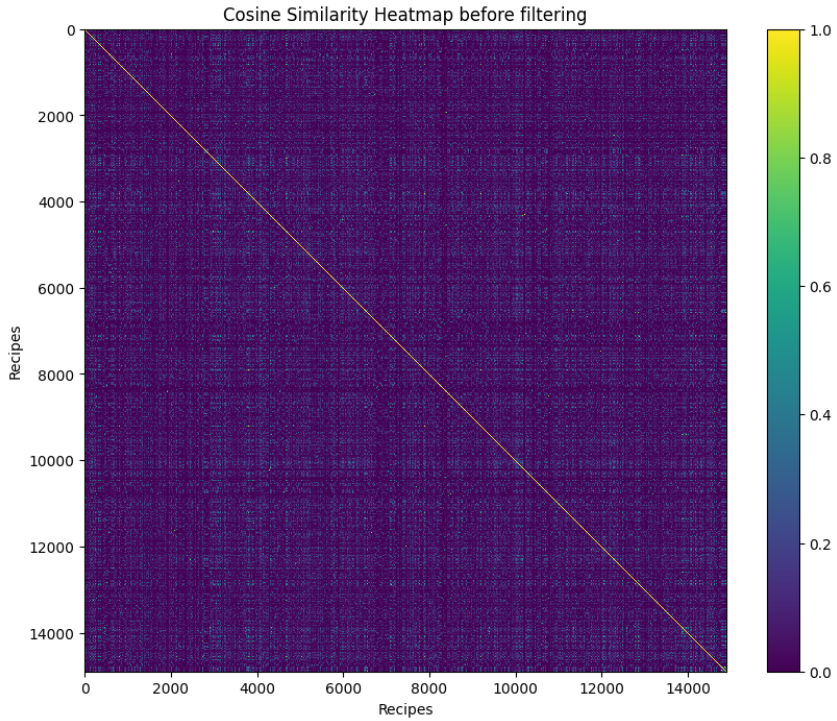
\includegraphics[width=0.4\textwidth]{7.png}
\caption{Cosine Similarity Heatmap before filtering}
\label{fig:monthly_publication}
\end{figure}

\begin{figure}[H]
\centering
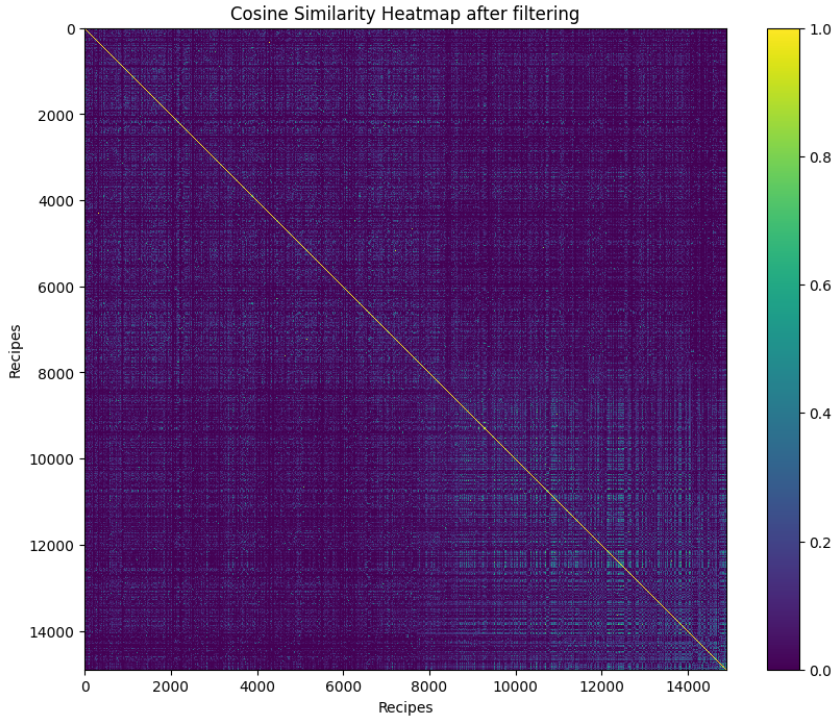
\includegraphics[width=0.4\textwidth]{8.png}
\caption{Cosine Similarity Heatmap after filtering}
\label{fig:monthly_publication}
\end{figure}

Here, we can see that the lighter region is increased after doing content-based filtering, proving that our algorithm is working correctly.

\section{Collaborative Filtering}

Collaborative filtering is a recommendation technique that identifies patterns in user behavior and preferences to recommend items to users. In this section, we describe the implementation of collaborative filtering for recipe recommendations using a reviewer-recipe-rating matrix.

\subsection{Creating Reviewer-Recipe-Rating Matrix}

A reviewer-recipe-rating matrix is constructed from the processed dataset, where each row represents a reviewer, each column represents a recipe, and the values represent the ratings given by reviewers to recipes. Missing ratings are filled with zeros.\\
Ratings may also be normalised to penalise ratings of those who ovverrate/underrate irratically.

\subsection{Calculating Cosine Similarity Matrix}

Cosine similarity is computed between reviewers based on their rating vectors using the reviewer-recipe-rating matrix. This similarity matrix captures the similarity between pairs of reviewers, indicating how alike their preferences are.

\subsection{Predicting Ratings for Missing Entries}

Predictions for missing ratings for each user are made one by one. This involves identifying similar users and using their ratings for the target recipe to predict missing rating. The predictions are based on the cosine similarity scores between users. 
\\
It is used to in a way to assign optimum weights to each other reviewer's rating. The users having rating vector similar to target user will have higher weight and vice versa. Weighted sum of these ratings is taken to predict target user's rating for the recipe.

\subsection{Printing Recommendations}
Recommendations for user = "Bergy":
\begin{itemize}
    \item Ham \&amp; Egg Casserole
    \item Shrimp Stir-Fry With Bok Choy, Mushrooms \& Pep...
    \item Perch or Snapper Fillet With Tomatoes and Onion
    \item Filet of Sole With Spinach \&amp; Tomatoes
    \item Turtle Cookies
\end{itemize}

\subsection{Analysis of results}
Used k-fold cross validation and then further divided val set into 2 parts. One that serves for predicting likes and dislikes. Other that serves as ground truth.\\

\begin{figure}[H]
\centering
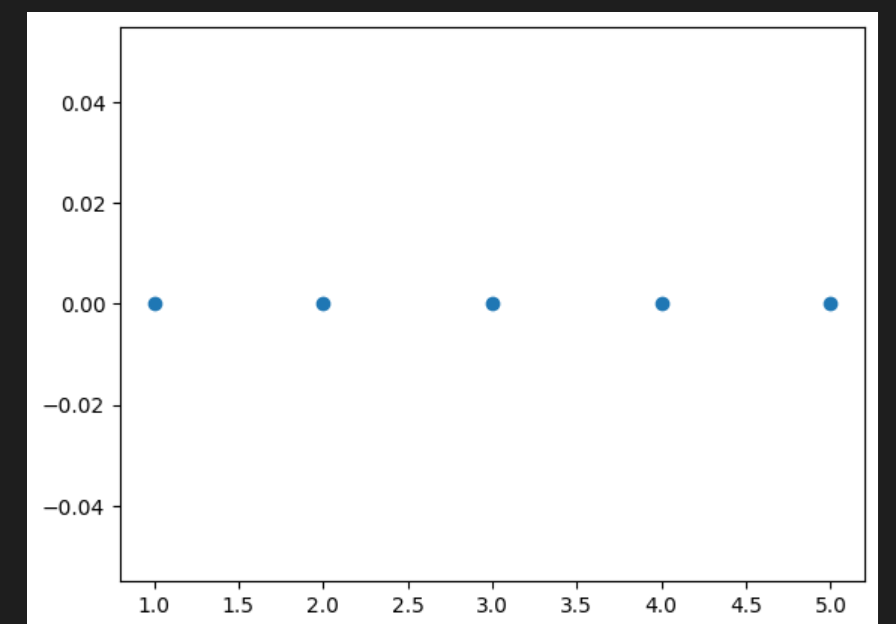
\includegraphics[width=0.4\textwidth]{Untitled.png}
\caption{Accuracy on various test datasets generated while applying cross validation}
\label{fig:Untitled}
\end{figure}


We got extremely poor results for accuracy as data is sparse in cosine similarity matrix. Most dishes being suggested are simply those which are liked by most as hardly any preference of users is matching due to sparseness.\\\\
Also, we are using the user's already rated dishes for ground truth. As most user have hardly tried any dishes, hence the suggested dishes (from among 14000 dishes) may not belong to the small set of ground truth anyways! There might exist many better dishes suited for user than the ones he has already tried (used as ground truth).\\
Hence, weights for each user's rating are not getting calculated as desired.\\\\
This issue might get rectified if all users have tried a lot of dishes. (User-Recipe-Rating matrix is not sparse)
\\
However this is unlikely to be a practical case in an actual food recommender system.

\section{K-Nearest Neighbors (KNN) Clustering}

\subsection{Introduction}
K-Nearest Neighbors (KNN) clustering is a popular machine learning technique used for recommendation systems. It works by finding the k nearest neighbors to a given data point based on a similarity metric, such as cosine similarity.

\subsection{Methodology}
In our recommendation system, we apply KNN clustering to identify recipes with similar ingredient profiles. The methodology involves preprocessing the dataset, vectorizing recipe ingredients using TF-IDF, and fitting a KNN model to find nearest neighbors.

\subsection{Example Recommendations}
We present below the example recommendations generated by the recommendation function using the K-Nearest Neighbors (KNN) clustering technique:

\subsubsection{For the Recipe 'Buttermilk Pie'}
\begin{itemize}
    \item Fried Cornbread II
    \item Easy Red Velvet Cake
    \item Chocolate Dessert Crepes
    \item Whole Wheat Buttermilk Rusks
    \item Sunrise Cherry Pie
\end{itemize}

\subsubsection{For the Recipe 'Potato Salad'}
\begin{itemize}
    \item Potatoes Tapas in Garlic Mayonnaise (Potatoes Aioli)
    \item Cold Picnic Potato Salad
    \item Quick Baked Potato
    \item Cheesy Hash Browns for One
    \item Irish Fadge (Potato Cakes)
\end{itemize}

These recommendations demonstrate the effectiveness of the K-Nearest Neighbors (KNN) clustering in providing relevant and diverse recipe suggestions based on ingredient similarity.

\subsection{Analysis of Results using Cosine Similarity Heatmap}

To analyze the effectiveness of the recommendation system, a cosine similarity heatmap is generated to visualize the pairwise similarities between recipes after applying content-based filtering.

The heatmap is generated using the cosine similarity matrix, where each cell represents the similarity score between two recipes. Lighter cells indicate higher similarity scores, suggesting that the corresponding recipes are more similar.

\begin{figure}[H]
\centering
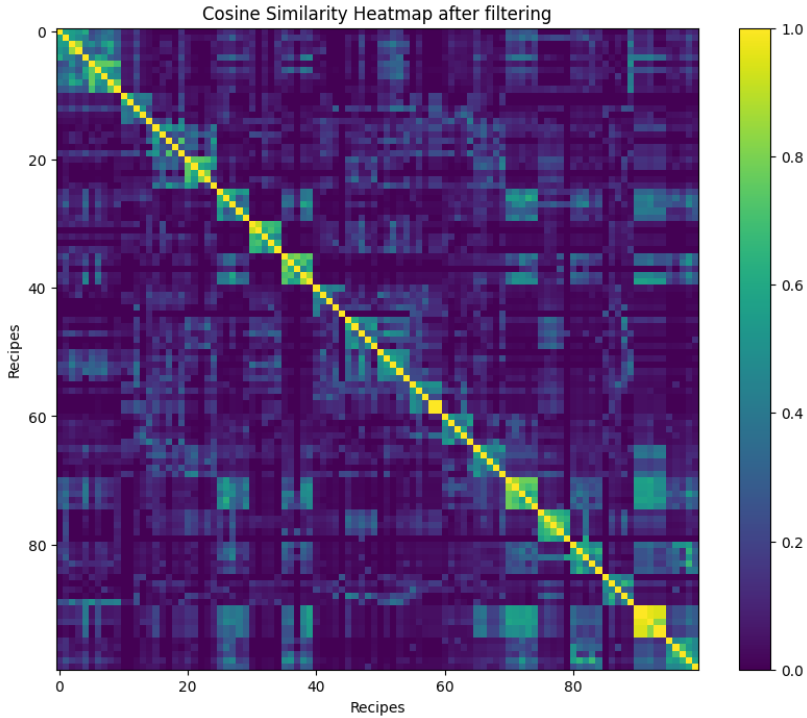
\includegraphics[width=0.4\textwidth]{9.png}
\caption{Heatmap after KNN clustering}
\label{fig:clustering}
\end{figure}

We can observe that squares of sides equal to cluster size are formed along the diagonal. This shows that clusters are created with similar recipes within then.

This analysis provides insights into how the content-based filtering affects the similarity structure of the recipe dataset and helps evaluate the quality of the recommendations.

\section{Neural Network}
Feedforward neural networks, also known as multilayer perceptrons (MLPs), are a fundamental type of neural network architecture. They consist of multiple layers of neurons, including an input layer, one or more hidden layers, and an output layer. Each neuron in a layer is connected to every neuron in the subsequent layer.
\\
In a feedforward neural network, information flows forward from the input layer through the hidden layers to the output layer without any feedback connections. Each neuron in the network computes a weighted sum of its inputs, applies an activation function to the result, and passes the output to the next layer.

\subsection{Scaling input data for training of NN}
We had to first scale data to the form that is required i.e. decimal and we also standardised the data.

\subsection{Define structure of NN}
We had to define hidden layers on NN. We chose after some experimenting having 2 hidden layers. 1st one having 32 nodes and 2nd one having 8. \\The output layer has only a single node representing the rating that has been predicted.

\subsection{MSE Loss}
We trained model for 5 epochs and plotted a graph for MSE.
\begin{figure}[H]
\centering
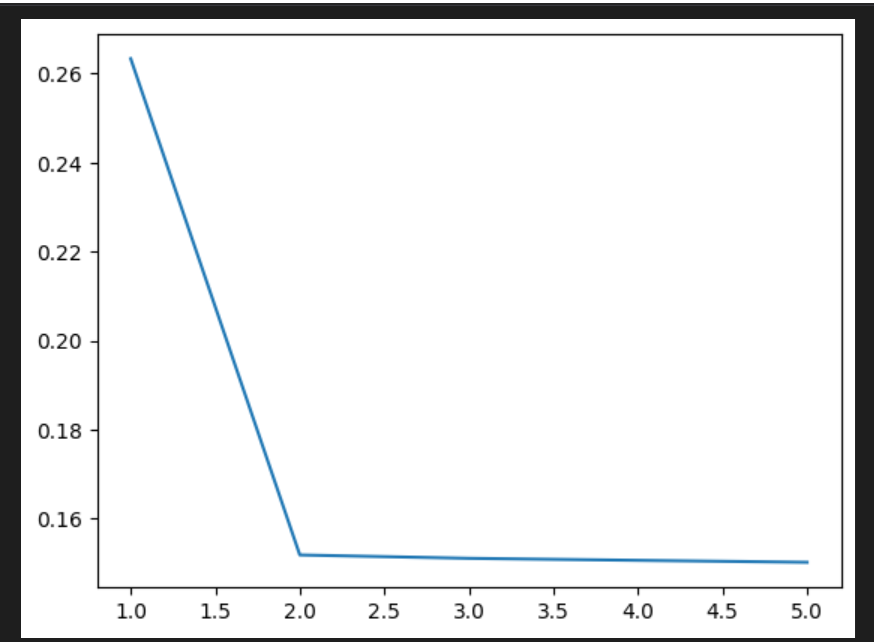
\includegraphics[width=0.4\textwidth]{Untitled2.png}
\caption{MSE Graph after training}
\label{fig:clustering}
\end{figure}

\subsection{Example Outputs}
For user ID = 1060485 ("allyop")
We recieved the following results :
\begin{itemize}
    \item Chicken Armenian
    \item Gracie Allen's Classic Roast Beef
    \item Italian Beef
    \item Old Fashioned Oatmeal Cookies
\end{itemize}

\section{Comparison and Conclusion}

Each recommendation method has its strengths and limitations. However, since we cannot directly compare them because this is a problem of unsupervised learning, we have listed their pros and cons. Also, the results can be manually confirmed by user testing, but this method is very exhaustive. Here are the details of each method:

\subsection{Collaborative Filtering}

Collaborative filtering excels in capturing user preferences and generating personalized recommendations. By analyzing user-item interaction data, it can identify similar users and recommend items based on their preferences. However, collaborative filtering may suffer from the cold start problem, where new users or items have limited interaction data. Additionally, the sparsity of user-item interaction data can affect the accuracy of recommendations.\\
This is the case with our dataset which results in extremely poor accuracy.

\subsection{Content-Based Filtering}

Content-based filtering leverages item features, such as ingredients in recipes, to provide recommendations based on item similarity. By analyzing the attributes of items, it can recommend items with similar attributes. However, content-based filtering may struggle with surprising or showing you something unexpected, as it primarily relies on the characteristics of items.

\subsection{K-Nearest Neighbors Clustering}

K-Nearest Neighbors clustering groups similar items and recommends items based on their neighbors within the same cluster. By identifying closely related items, it can provide recommendations based on item similarity. However, KNN clustering may not capture diverse recommendations, as it tends to recommend items within the same cluster.

\subsection{Deep Learning}

Deep learning is the most advanced technique known till date. It has the potential to learn complex patterns and representations from data, leading to highly accurate and personalized recommendations. However, deep learning models require large amounts of data and computational resources for training, making them challenging to deploy in real-world applications.\\
We find that NN works quite well with out dataset and also shows significantly less error.

\subsection{Conclusion}

In conclusion, each recommendation method offers unique advantages and challenges. A hybrid approach that combines multiple methods can overcome individual limitations and enhance recommendation quality. Furthermore, manual confirmation through user testing can validate the effectiveness of recommendation methods in real-world scenarios. Future research may focus on developing hybrid recommendation systems and exploring advanced techniques to address specific challenges in recommendation systems.\\
In our manual trial runs based on various dishes and users, we find that potentially due to sparsity of rating data, the Content based Filtering and Neural Network methods work the best.

% Individual Contribution
\section{Individual Contributions}
\subsection{Himang Chandra Garg}
\begin{itemize}
    \item Implemented data visualization techniques using Matplotlib and Seaborn libraries.
    \item Developed the content-based filtering algorithm using TF-IDF vectorization and cosine similarity.
    \item Used the K-Nearest-Neighbour approach to recommend based on clusters.
    \item Showed that the above techniques give similar results by plotting the graph of Cosine similarity Heatmap.
\end{itemize}

\subsection{Nishil Agarwal}
\begin{itemize}
    \item Implemented data preprocessing pipeline, including filtering, cleaning, and formatting of the dataset.
    \item Developed the collaborative filtering algorithm for generating user-based recommendations by using cosine similarity matrix.
    \item Showed accuracy results through k-fold cross validation and sub-sampling on collaborative filtering
    \item Developed Neural Network method and generated accuracy graphs for it.
\end{itemize}

% References
\begin{thebibliography}{99}
\bibitem{reference1}
https://www.kaggle.com/datasets/irkaal/foodcom-recipes-and-reviews
\item https://www.nature.com/articles/s41598-022-10358-x
\item https://a-elkhattam.medium.com/imdb-movie-recommendation-chatbot-942f84dfa0dc
\item https://www.analyticsvidhya.com/blog/2020/10/quick-guide-to-evaluation-metrics-for-supervised-and-unsupervised-machine-learning/
\item https://www.geeksforgeeks.org/cross-validation-machine-learning/
\item https://medium.com/@azadmeshram/evaluation-of-collaborative-filtering-model-6559b1a49b77
\item https://prabhatm27.medium.com/creating-a-hybrid-neural-network-for-movie-recommendations-using-tensorflow-recommenders-fdad13aa4979
\item https://pythonprogramming.net/introduction-deep-learning-python-tensorflow-keras/
\end{thebibliography}


\end{document}
